\section{implementacja}

\subsection{Technologia}
Podstawowym założeniem projektu było stworzenie nowoczesnej aplikacji desktopowej,
która zintegrowałaby wiele funkcji, takich jak dostęp do bazy danych, nowoczesny interfejs,
i prostotę implementacji. 

Projket zaimplementowany został w technologii Electron JS.

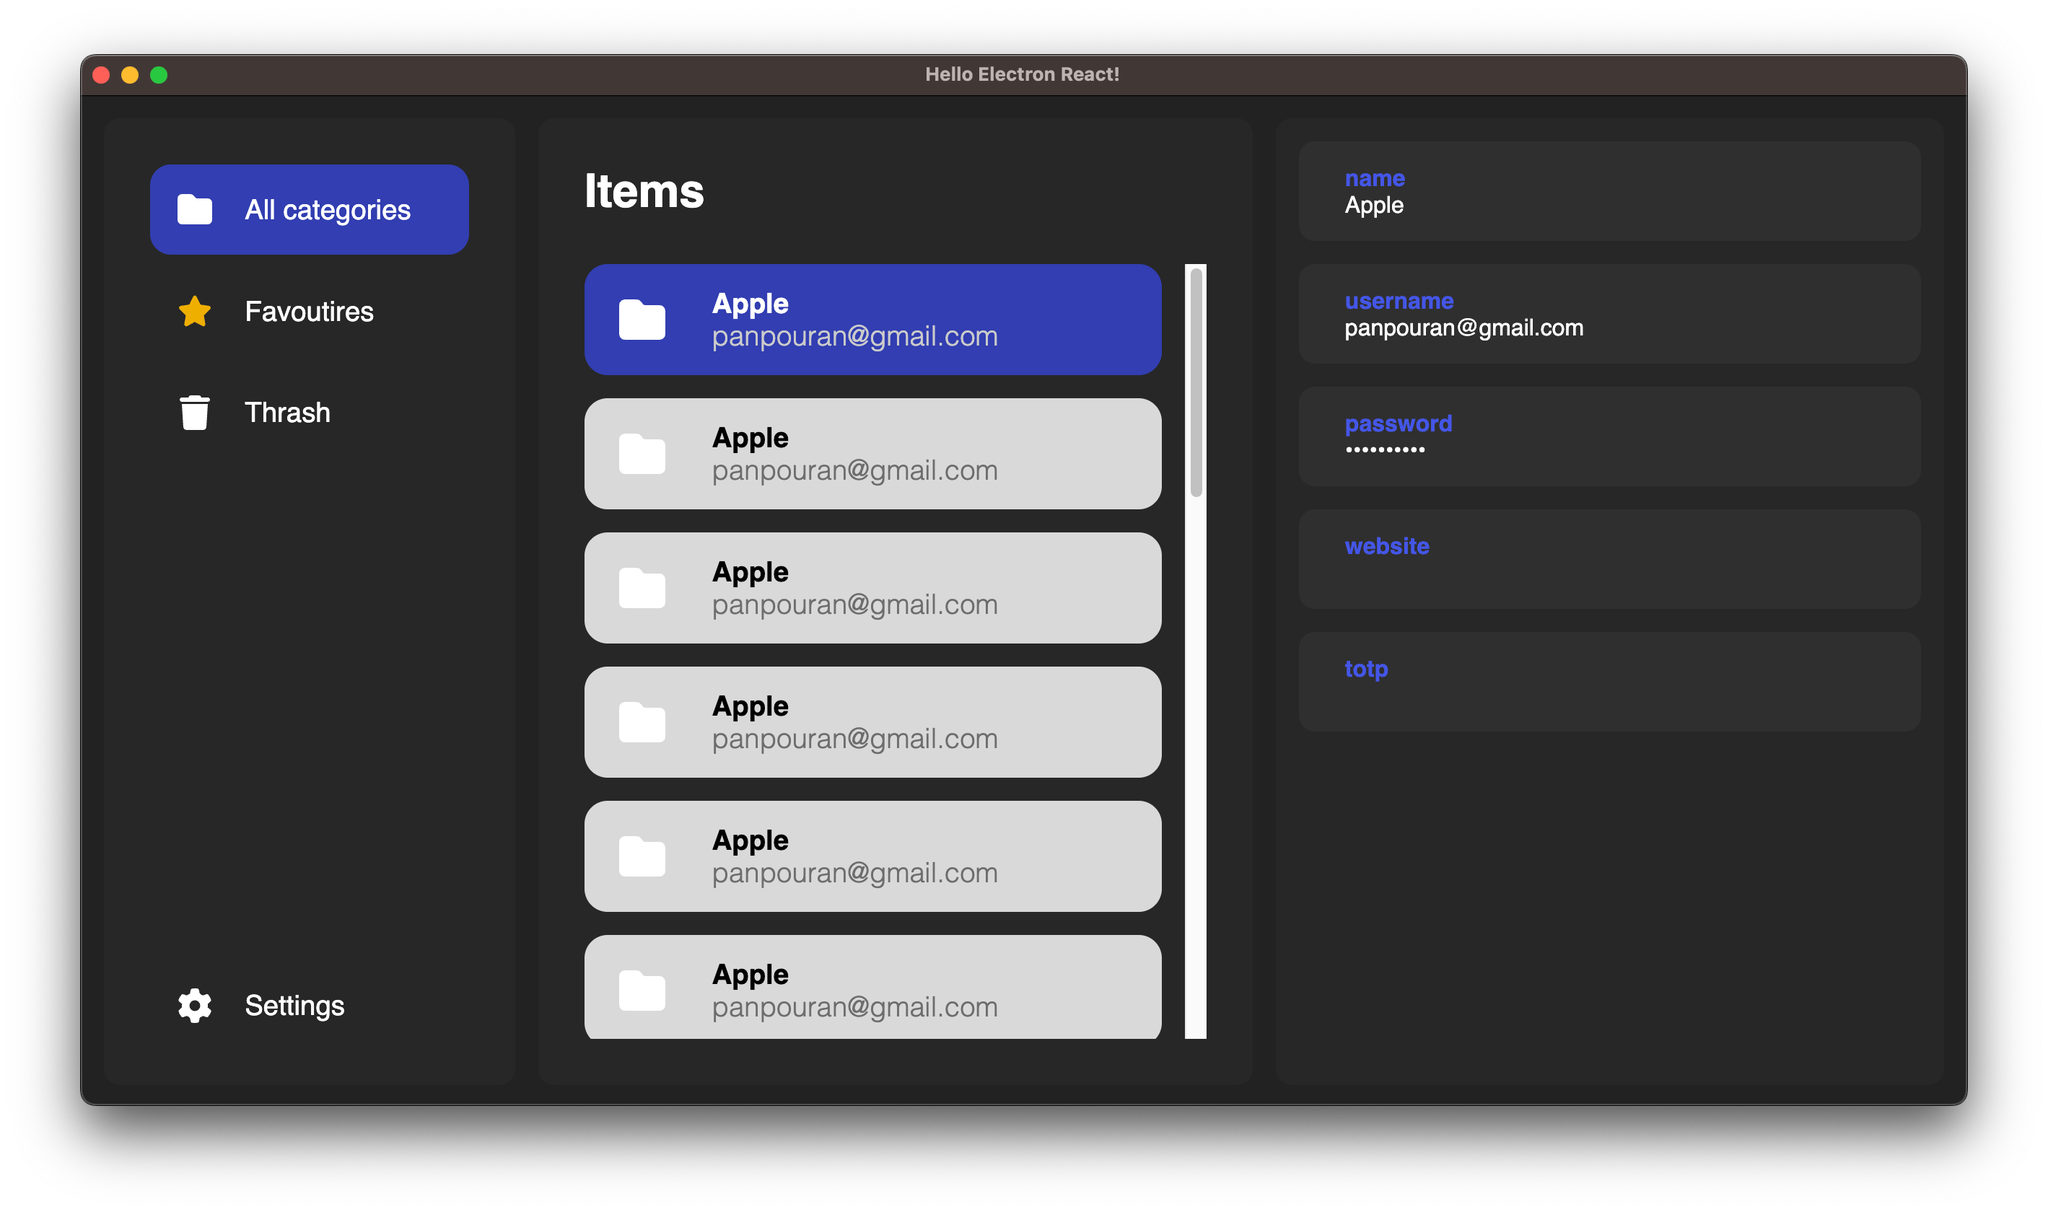
\includegraphics[width=1\linewidth]{interfejs}
\subsection{Szczegóły implementacji szyfrowania}
Szyfrowanie danych składa się z:
\begin{itemize}
    \item Utworzenie soli (salt) unikalny, losowy ciąg znaków, dodawany do hasła przed jego haszowaniem. (Zabezpieczenie przed atakami 'rainbow tables'),
    \item Wytworzenie  klucza kryptograficznego przy użyciu funkcji skrótu PBKDF2 z podanym hasłem głównym  i salt. (z użyciem 100 000 iteracji),
    \item Utworzenie wektora inicjalizującego,
    \item Szyfrowanie  danych  algorytmem AES-256-CBC z użyciem klucza oraz wektora inicjalizującego,
\end{itemize}
Deszyfrowanie danych składa się z:
\begin{itemize}
    \item Wytworzenie  klucza kryptograficznego w sposób taki jak w mechanizmie szyfrowania
    \item Odszyfrowanie  danych  algorytmem AES-256-CBC z użyciem klucza oraz wektora inicjalizującego
\end{itemize}
Poniższy kod pokazuje jak zaimplementowane zostało szyforwanie oraz deszyfrowanie danych w aplikacji:

\includegraphics*[width=0.8\linewidth]{kod}



